% -----------------------------------------------------------------------
% -----------------------------------------------------------------------
\section*{Aufbau}
% Zell: Kapitel 7.1
Es gibt eigentlich historisch gesehen nicht \textit{das} Perzeptron, sondern eine ganze Familie verwandter Modelle neuronaler Netze, die von Frank Rosenblatt Anfang der 60er Jahre entwickelt wurden und die alle mit Perzeptron bezeichnet wurden.

Ein allgemeines Perzeptron hat folgenden Aufbau (Vgl. Abbildung \ref{fig:perzeptron-minsky-papert}):
\begin{itemize}
	\item \emph{Schicht mit Eingabezellen} \\
	Retina - Dient der reinen Datenaufnahme (Muster) und hat festgewichtete Verbindungen zur nächsten Neuronenschicht. (Diese Schicht wird im Folgenden oftmals nicht dargestellt.)
	
	\item \emph{Schicht mit Neuronen} \\
	Eingabeschicht - Neuronen ohne Informationsverarbeitung jedoch mit trainierbaren Verbindungen zum Ausgabeneuron.

	\item Ausgabeneuron $\Omega$ \\
	Klassifikator - Neuron mit Informationsverarbeitung, welches angibt, ob das an der Retina anliegende Muster vom Perzeptron erkannt wird oder nicht.
\end{itemize}

\begin{figure}[ht!] \centering 
	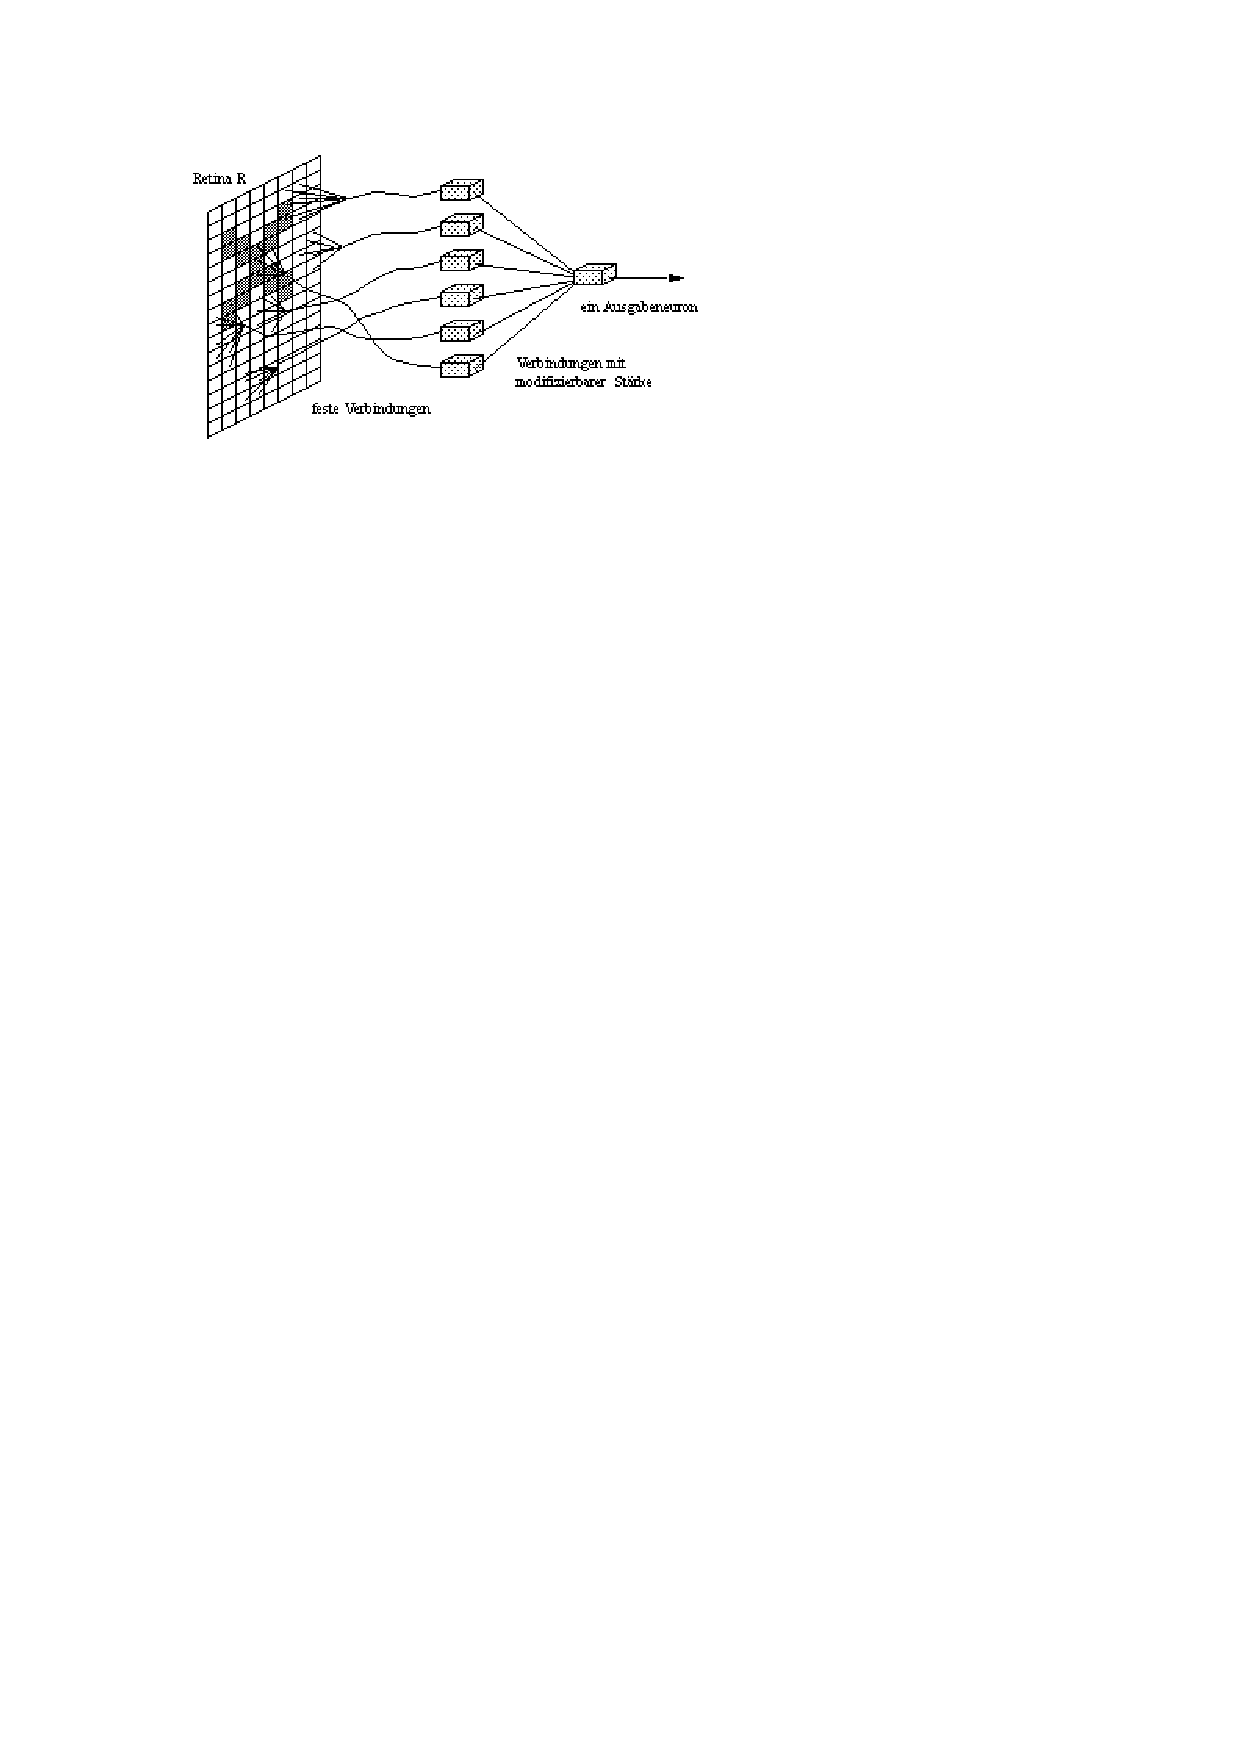
\includegraphics[width=\linewidth]{figures/ch02_perzeptron-minsky-papert.pdf}
	\caption{Struktur des Perzeptron nach Minsky und Papert.}
	\label{fig:perzeptron-minsky-papert}
\end{figure}

Weiterhin wird unter dem Begriff \emph{Perzeptron} oft das binäre Modell des Perzeptrons verstanden, bei dem die Eingaben und die Aktivierungen der Neuronen nur binäre Werte 0 und 1 (bzw. -1 und 1) annehmen dürfen. Die Gewichte können allerdings beliebige reelle Werte annehmen.

% -----------------------------------------------------------------------
\subsection*{Neuronen des Perzeptrons}
% Zell: Kapitel 7.2
Die Neuronen der Eingabeschicht werden in diesem Modell nicht spezifiziert. Es genügt, wenn man sie als \emph{binäre Eingaben} betrachtet.
Damit kann das Schema eines Perzeptrons wie in Abbildung \ref{fig:perzeptron-schema} links dargestellt werden. Dabei ist jedes Neuron der Ebene 0 fest mit allen Neuronen der Eingabeschicht verbunden.

\begin{figure}[ht!] \centering 
	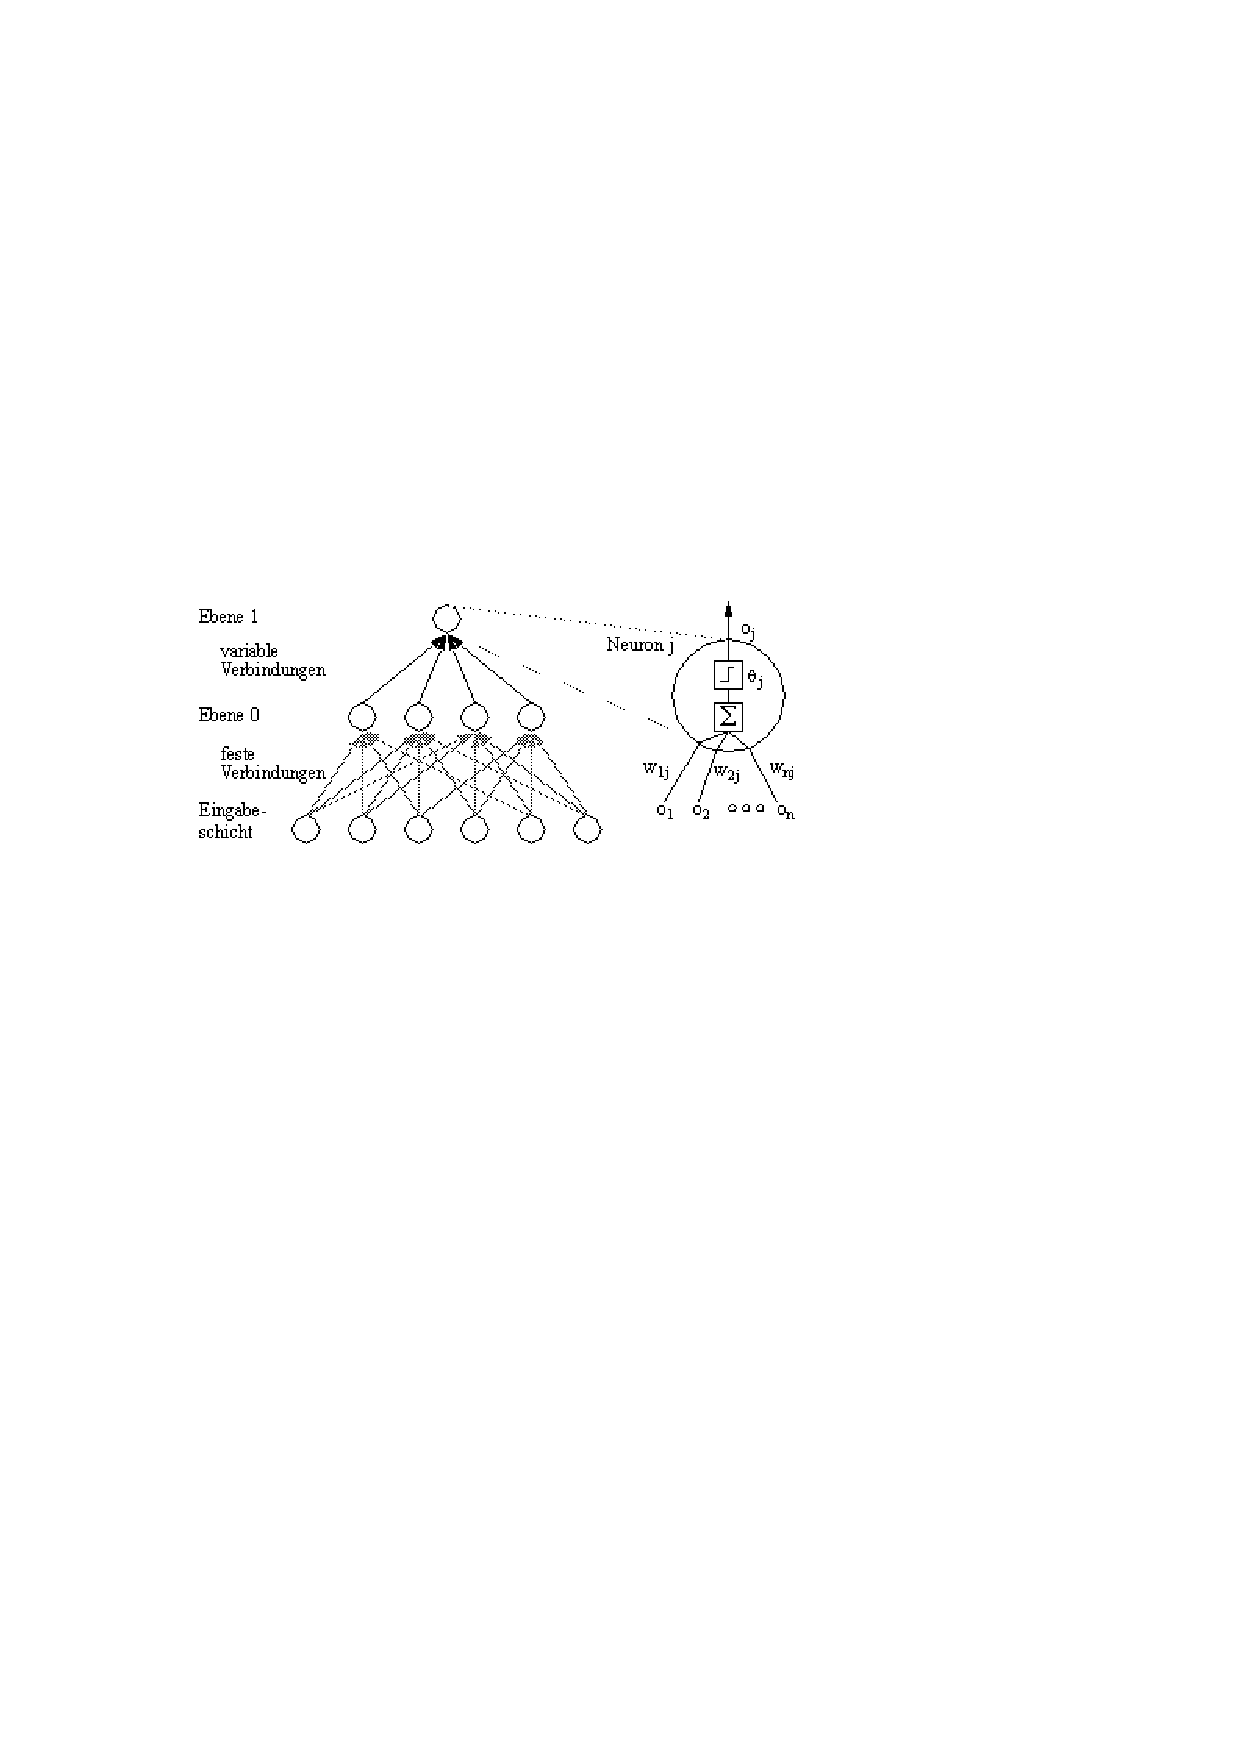
\includegraphics[width=\linewidth]{figures/ch02_perzeptron-schema.pdf}
	\caption{Schema des Perzeptrons (links) und Ausgabeneuron des Perzeptrons (rechts).}
	\label{fig:perzeptron-schema}
\end{figure}

Jedes Neuron der Ebenen 0 und 1 des Perzeptrons hat das in Abbildung \ref{fig:perzeptron-schema} rechts dargestellte Verhalten: Es summiert seine Eingaben auf ($net_j$), die sich als Ausgaben der Vorgängerneuronen ($o_i$) multipliziert mit dem jeweiligen Gewicht $w_{ij}$ ergeben: 
\[
	net_j = \sum_i o_i \cdot w_{ij}
\]

 Auf diese Netzeingabe $net_j$ wird eine binäre Schwellenwertfuktion angewandt: Die Ausgabe $o_j$ ist 1, falls die Netzeingabe größer oder gleich dem Schwellenwert $\theta_j$ ist, andernfalls ist die Ausgabe 0:
\[
	o_j = a_j = 
	\begin{cases}
		1 &\text{falls } net_j \ge \theta_j \\
		0 &\text{sonst}
	\end{cases}
\]

% -----------------------------------------------------------------------
\subsection*{Repräsentierbarkeit und Lernfähigkeit}

\subsubsection*{Repräsentierbarkeit} 
Repräsentierbarkeit bezeichnet die Fähigkeit eines Netzes, eine gegebene Funktion (Prädikat) mit dem neuronalen Netz realisieren zu können. Hierbei ist die Topologie des Netzes vorgegeben, es dürfen aber alle Gewichte und Schwellenwerte korrekt bzw. optimal gewählt werden.

\subsubsection*{Lernfähigkeit} 
Lernfähigkeit ist die Fähigkeit eines Lernalgorithmus, ein Netzwerk eine repräsentierbare Funktion (Prädikat) lernen zu lassen. D.h. die Gewichte und Schwellenwerte durch den \emph{Algorithmus} korrekt zu bestimmen. \\

Die Unterscheidung zwischen Repräsentierbarkeit und Lernfähigkeit ist sehr wichtig\footnote{Die Unterscheidung ist auch aus historischen Gründen sehr wichtig, weil sie in der ersten Blütephase neuronaler Netze noch nicht bekannt war und daher ein berühmtes Theorem, das Perzeptron-Lern-Theorem von F. Rosenblatt über die Fähigkeit des Perzeptron-Lernalgorithmus, meist falsch verstanden wurde.}:
\emph{Repräsentierbarkeit} stellt eine Fähigkeit des Netzes dar und ist nur von der Topologie und den gewählten Aktivierungs- und Ausgabefunktionen des Netzes abhängig, jedoch unabhängig von einem gewählten Lernalgorithmus.
\emph{Lernfähigkeit} hingegen ist eine Eigenschaft eines speziellen Lernalgorithmus. 



% -----------------------------------------------------------------------
% -----------------------------------------------------------------------
\section*{Lineare Trennbarkeit}
% Zell: Kapitel 7.3
Das Konzept der linearen Trennbarkeit kann man am besten an einem einfachen Beispiel, dem bekannten XOR-Problem, demonstrieren. Man betrachte hierzu ein einstufiges Perzeptron-Netzwerk mit einem Ausgabeneuron $j$ in Ebene 1 und zwei Neuronen in Ebene 0. Die Ausgabe des Neurons $j$ soll 0 sein, falls seine binären Eingaben gleich sind ($o_1 = o_2$) sonst soll sie 1 sein. Das heißt, damit $o_j = 1$ ist, muss gelten:
\[
	net_j = o_1 w_{1j} + o_2 w_{2j} \ge \theta_j
\]
Für $w_{2j} \ge 0$ ist dies äquivalent zu der Ungleichung
\[
	o_2 \ge \frac{1}{w_{2j}} ( \theta_j - o_1 w_{1j})
\]
Für einen konstanten Schwellwert $\theta_j$ ergibt sich also eine Gerade in der durch $o_1$ und $o_2$ gebildeten Ebene (siehe Abbildung \ref{fig:lineare-separierbarkeit}). Alle Punkte oberhalb dieser Geraden stellen bei positivem $w_{2j}$ Kombinationen von $o_1$ und $o_2$ dar, für die das Neuron feuert. Bei negativem $w_{2j}$ sind alle Punkte unterhalb der Geraden Punkte, für die das Neuron feuert.

\begin{figure}[ht!] \centering 
	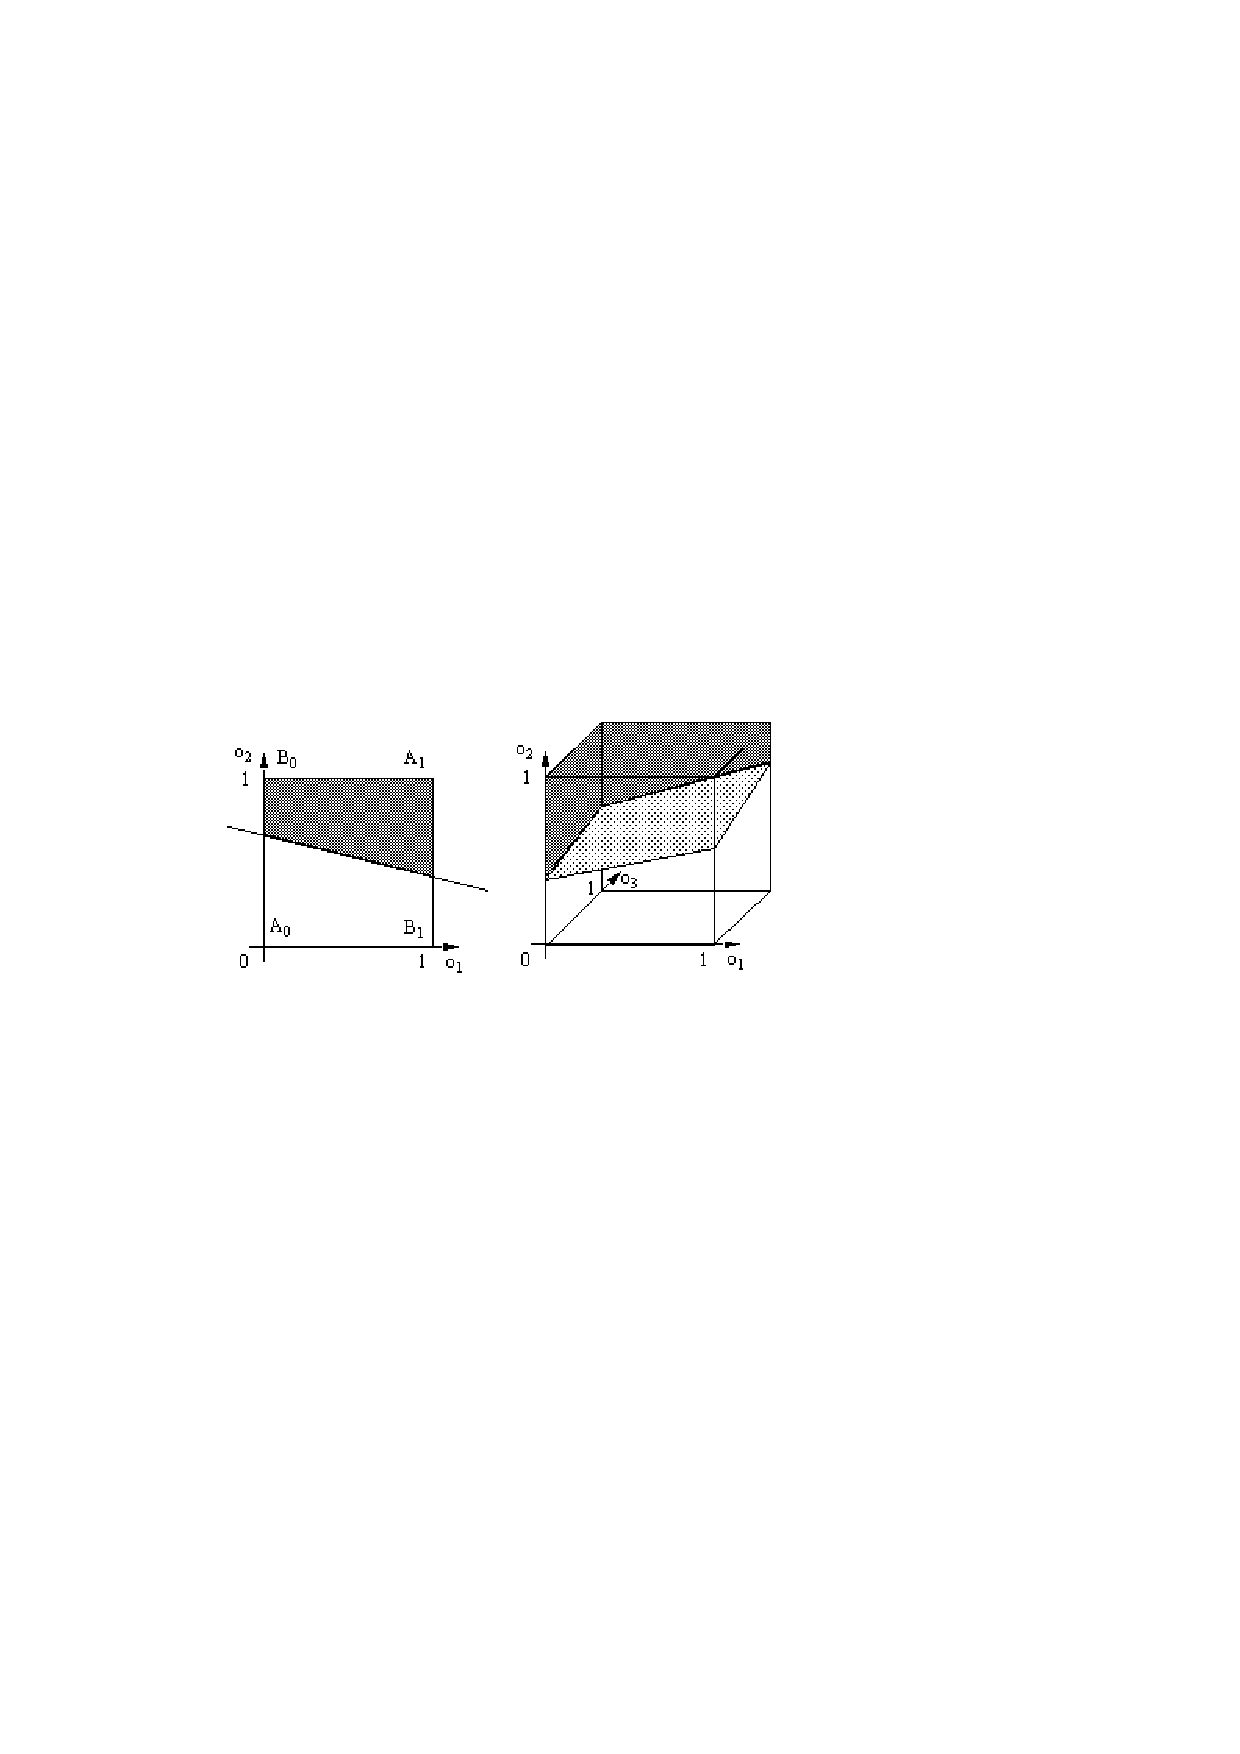
\includegraphics[width=\linewidth]{figures/ch02_lineare-trennbarkeit.pdf}
	\caption{Lineare Trennbarkeit und das XOR-Problem.}
	\label{fig:lineare-separierbarkeit}
\end{figure}

Ein neuronales Netz, welches das XOR-Problem lösen will, muss die Punkte $A_0 (0|0)$ und $A_1 (1|1)$ einer Klasse A zuordnen, die Punkte $B_0 (0|1)$ und $B_1 (1|0)$ der Klasse B. Diese Trennung ist mit einer einzigen Gerade, welche den Eingabereaum linear trennt, nicht möglich. 
Deshalb gilt: Die Menge $A = \{A_0, A_1\}$ und $B = \{B_0, B_1\}$ des XOR-Problems sind nicht linear separierbar, d.h. es gibt keine Wertekombination von $w_{1j}$, $w_{2j}$ und $\theta_j$, für die $net_j < \theta_j$ für alle Punkte in A und zugleich $net_j \ge \theta_j$ für alle Punkte in B ist.

Bei $n$ Eingängen eines Neurons, kann man den Raum der Eingaben als n-dimensionalen Würfel darstellen (sofern die Eingaben auf $[0,1]$ beschränkt ist, sonst ist es der n-dimensionale Raum).
Das Neuron trennt diesen Eingaberaum durch eine $(n-1)$-dimensionale \emph{Hyperebene}. Für $n=3$ ist dies in Abbildung \ref{fig:lineare-separierbarkeit} dargestellt.

Allgemein gilt: Ein einstufiges Perzeptron (d.h. ein Perzeptron mit nur einer Stufe modifizierbarer Gewichte) kann nur linear separierbare Mengen, d.h. Mengen, die durch eine Hyperebene trennbar sind, klassifizieren.


% -----------------------------------------------------------------------
\subsection*{Entscheidungsfunktion $g(x)$}
Eine Entscheidungsfunktion weißt einem Eingabevektor $\vec{x}$ eine der $k$ Klassen zu. Diese Klasse wird als $C_k$ bezeichnet.
Es seien folgende Werte gegeben:
\begin{align*}
	& \vec{x} = (x_1, \ldots, x_n)^T &\text{Merkmalsvektor} \\
	& \vec{w} = (w_1, \ldots, w_n)^T &\text{Gewichtsvektor} \\
	& w_0	&\text{Bias/Threshold}
\end{align*}

\subsubsection*{Zwei Klassen}
Bei $k=2$ gilt die einfachste Form der Entscheidungsfunktion $g(x)$:
\[
	g(\vec{x}) = \sum_{i=1}^{n} w_i x_i + w_0 = \vec{w}^T \vec{x} + w_0
\]
Der Merkmalsvektor $\vec{x}$ wird der Klasse $C_1$ zugeordnet wenn $g(\vec{x}) \ge 0$, andernfalls wird er der Klasse $C_2$ zugeordnet. Die Entscheidungsfunktion $g(x)$ gibt den Abstand zwischen Entscheidungsgrenze und Merkmalsvektor zurück. 

Die Entscheidungsgrenze ist damit für $g(\vec{x}) = 0$ definiert. Sie entspricht einer $(d-1)$-dimensionalen Hyperebene innerhalb eines $d$-dimensionalen Merkmalsraums und wird mit $H$ bezeichnet:
\[
	H: g(\vec{x}) = \sum_{i=1}^{n} w_i x_i + w_0 = \vec{w}^T \vec{x} + w_0 = 0
\]
Der normierte Vektor $\vec{w}$ gibt die Richtung und der Bias $w_0$ die Lage dieser Entscheidungsgrenze an. Die Hpyerebene $H$ trennt den Merkmalsraum in zwei Hälften auf; Entscheidungsregion $R_1$ für $C_1$ und $R_2$ für $C_2$. Liegt $\vec{x}$ in $R_1$ ($g(x) \ge 0$), zeigt auch der Normalenvektor $\vec{w}$ in $R_1$. Abbildung \ref{fig:lineare-entscheidunsfunktion} zeigt dies. Für den Abstand $r$ zwischen Hyperebene $H$ und Merkmalsvektor $\vec{x}$ gilt:
\[
	r = \frac{g(x)}{||w||}
\]

\begin{figure}[ht!] \centering 
	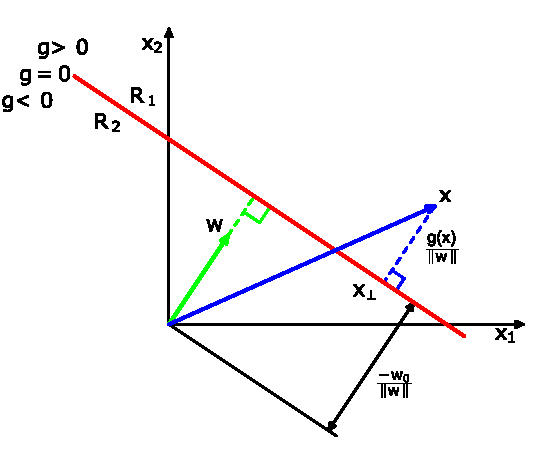
\includegraphics[width=\linewidth]{figures/ch02_lineare-entscheidungsfunktion.pdf}
	\caption{Grafisches Schaubild zur linearen Entscheidungsfunktion $g(x)$ in einem zweidimensionalen Merkmalsraum.}
	\label{fig:lineare-entscheidunsfunktion}
\end{figure}


\subsubsection*{Mehrere Klassen}
Bei $k > 2$ Klassen gibt es verschiedene Möglichkeiten eine k-Klassen-Diskriminantfunktion durch Kombinationen von Zwei-Klassen-Diskriminantfunktionen zu bestimmen:
\begin{itemize}
 	\item \emph{one-versus-the-rest} \\
 	$k-1$ Klassifikatoren die alle jeweils ein Zwei-Klassen-Problem lösen: Sie trennen Punkte, die zur Klasse $C_k$ gehören von Punkten, die nicht zu $C_k$ gehören (siehe Abbildung \ref{fig:lineare-entscheidungsfunktion-mehrere-klassen} oben).

 	\item \emph{one-versus-one} \\
 	Bei diesem Ansatz gibt es $\frac{k(k-1)}{2}$ binäre Diskriminantfunktionen: Eine für jedes mögliche Klassenpaar (siehe Abbildung \ref{fig:lineare-entscheidungsfunktion-mehrere-klassen} unten). 
 \end{itemize} 

\begin{figure}[ht!] \centering 
	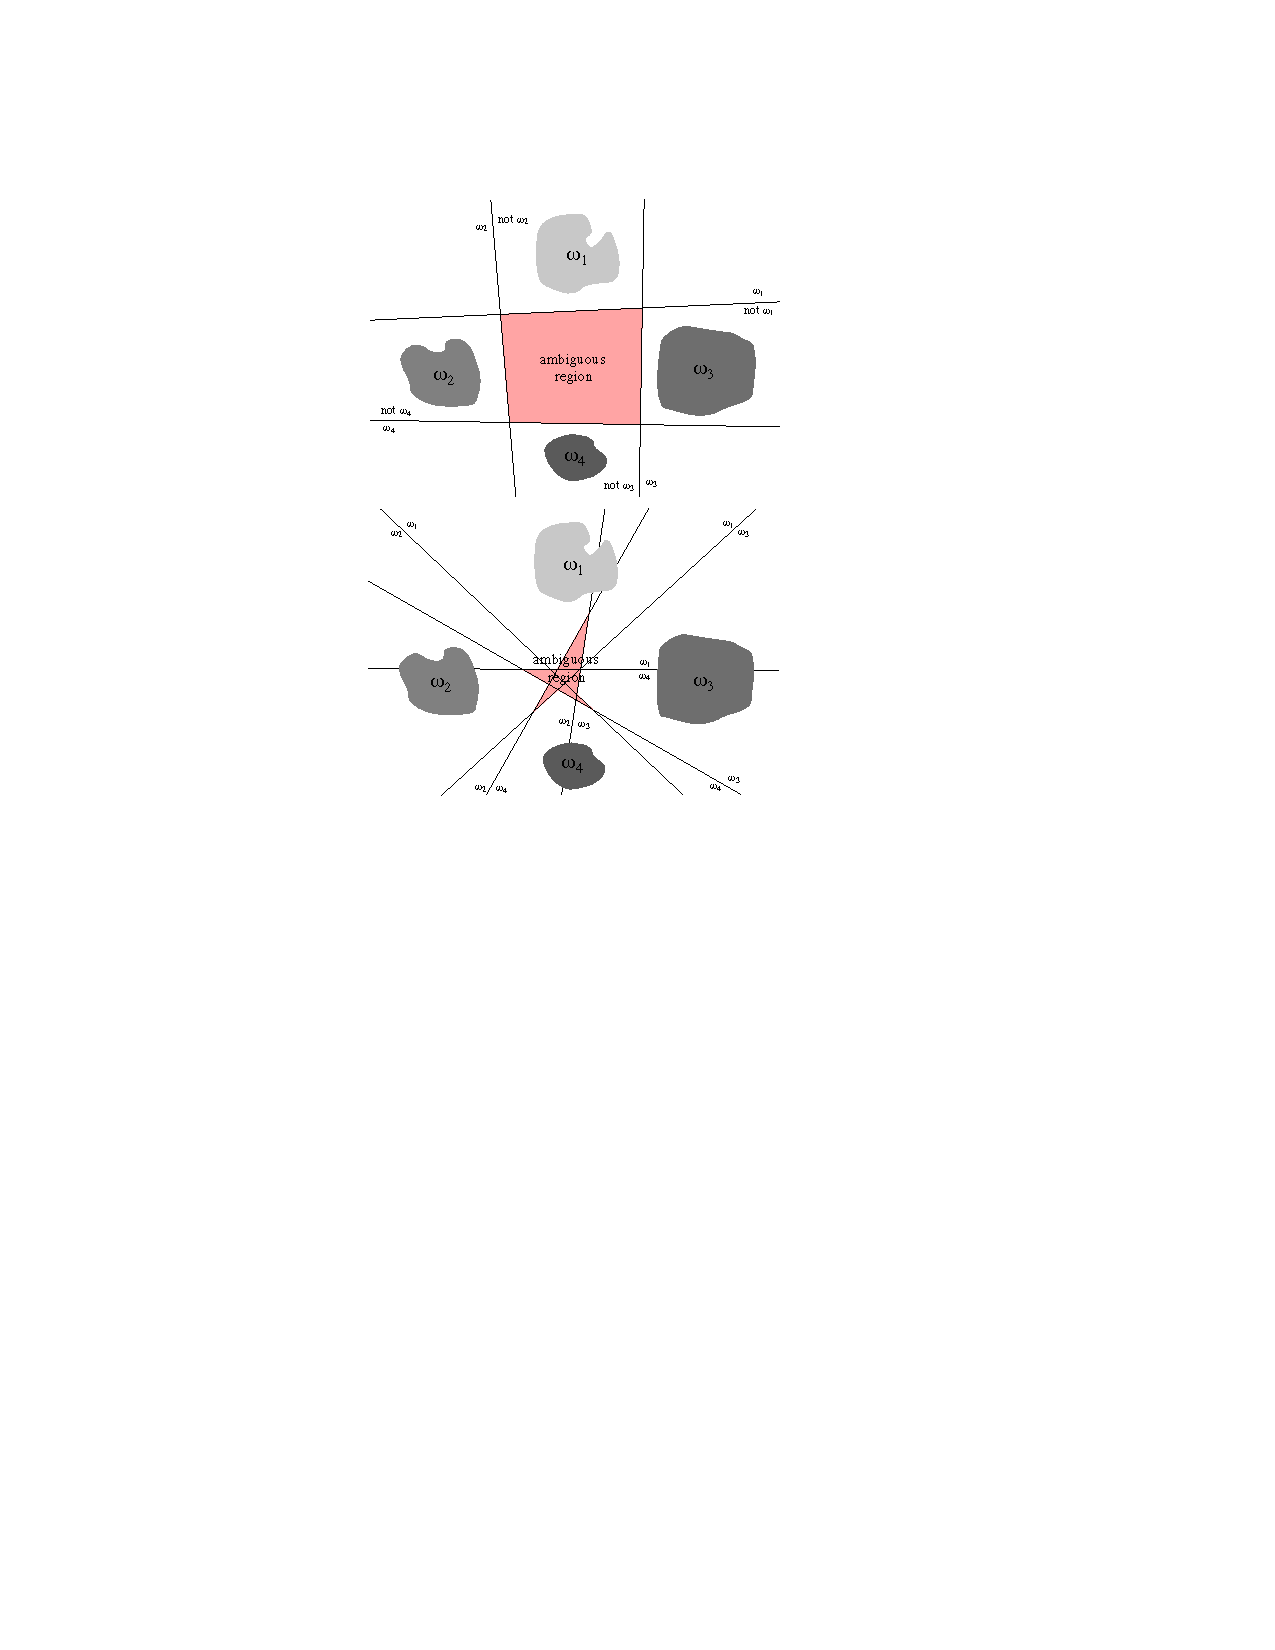
\includegraphics[width=\linewidth]{figures/ch02_lineare-entscheidungsfunktion-mehrere-klassen.pdf}
	\caption{Lineare Entscheidungsgrenzen für ein 4-Klassen-Problem. Oben der \emph{one-versus-the-rest} Ansatz ($C_i$ oder nicht $C_i$). Unten der \emph{one-versus-one} Ansatz ($C_i$ oder $C_j$ für alle $j \ne i$)}
	\label{fig:lineare-entscheidungsfunktion-mehrere-klassen}
\end{figure}

Beide Vorgehensweisen führen jedoch zu Bereichen des Merkmalsraums, welche nicht eindeutig einer Klasse zugeordnet werden können (in Abbildung \ref{fig:lineare-entscheidungsfunktion-mehrere-klassen} farbig hervorgehoben).
Deshalb wird für den Fall dass $k > 2$ ist der Ansatz der Entscheidungsfunktion für zwei Klassen wie folgt erweitert:
\[
	g_k(\vec{x}) = \vec{w}_k^T\vec{x} + w_{k0}
\]
Der daraus resultierende Klassifikator wird \emph{linear machine} genannt und teilt den Merkmalsraum in $k$ Entscheidungsregionen auf (siehe Abbildung \ref{fig:linear-machine}. Dabei ist $g_k(\vec{x})$ die größte Diskriminante, wenn $x$ in der Region $R_k$ liegt. Demnach wird der Merkmalsvektor $\vec{x}$ der Klasse $C_k$ zugeordnet, wenn gilt:
\[
	g_k(\vec{x}) > g_j(\vec{x}) \qquad \text{für alle } j \ne k
\]
Die Entscheidungsgrenze zwischen Klasse $C_k$ und Klasse $C_j$ ist gegeben für $g_k(\vec{x}) = g_j(\vec{x})$. Daraus folgt, analog zur Entscheidungsgrenze für den Zwei-Klassen-Fall, eine $(d-1)$-dimensionale Hyperebene, für die gilt:
\[
	(\vec{w}_k - \vec{w}_j)^T x + (w_{k0} - w_{j0}) = 0
\]
Im Gegensatz zur Entscheidungsgrenze im Zwei-Klassen-Fall ist hier nicht der Gewichtsvektor $\vec{w}$ entscheidend, sondern die Differenz $\vec{w}_k - \vec{w}_j$.

\begin{figure}[ht!] \centering 
	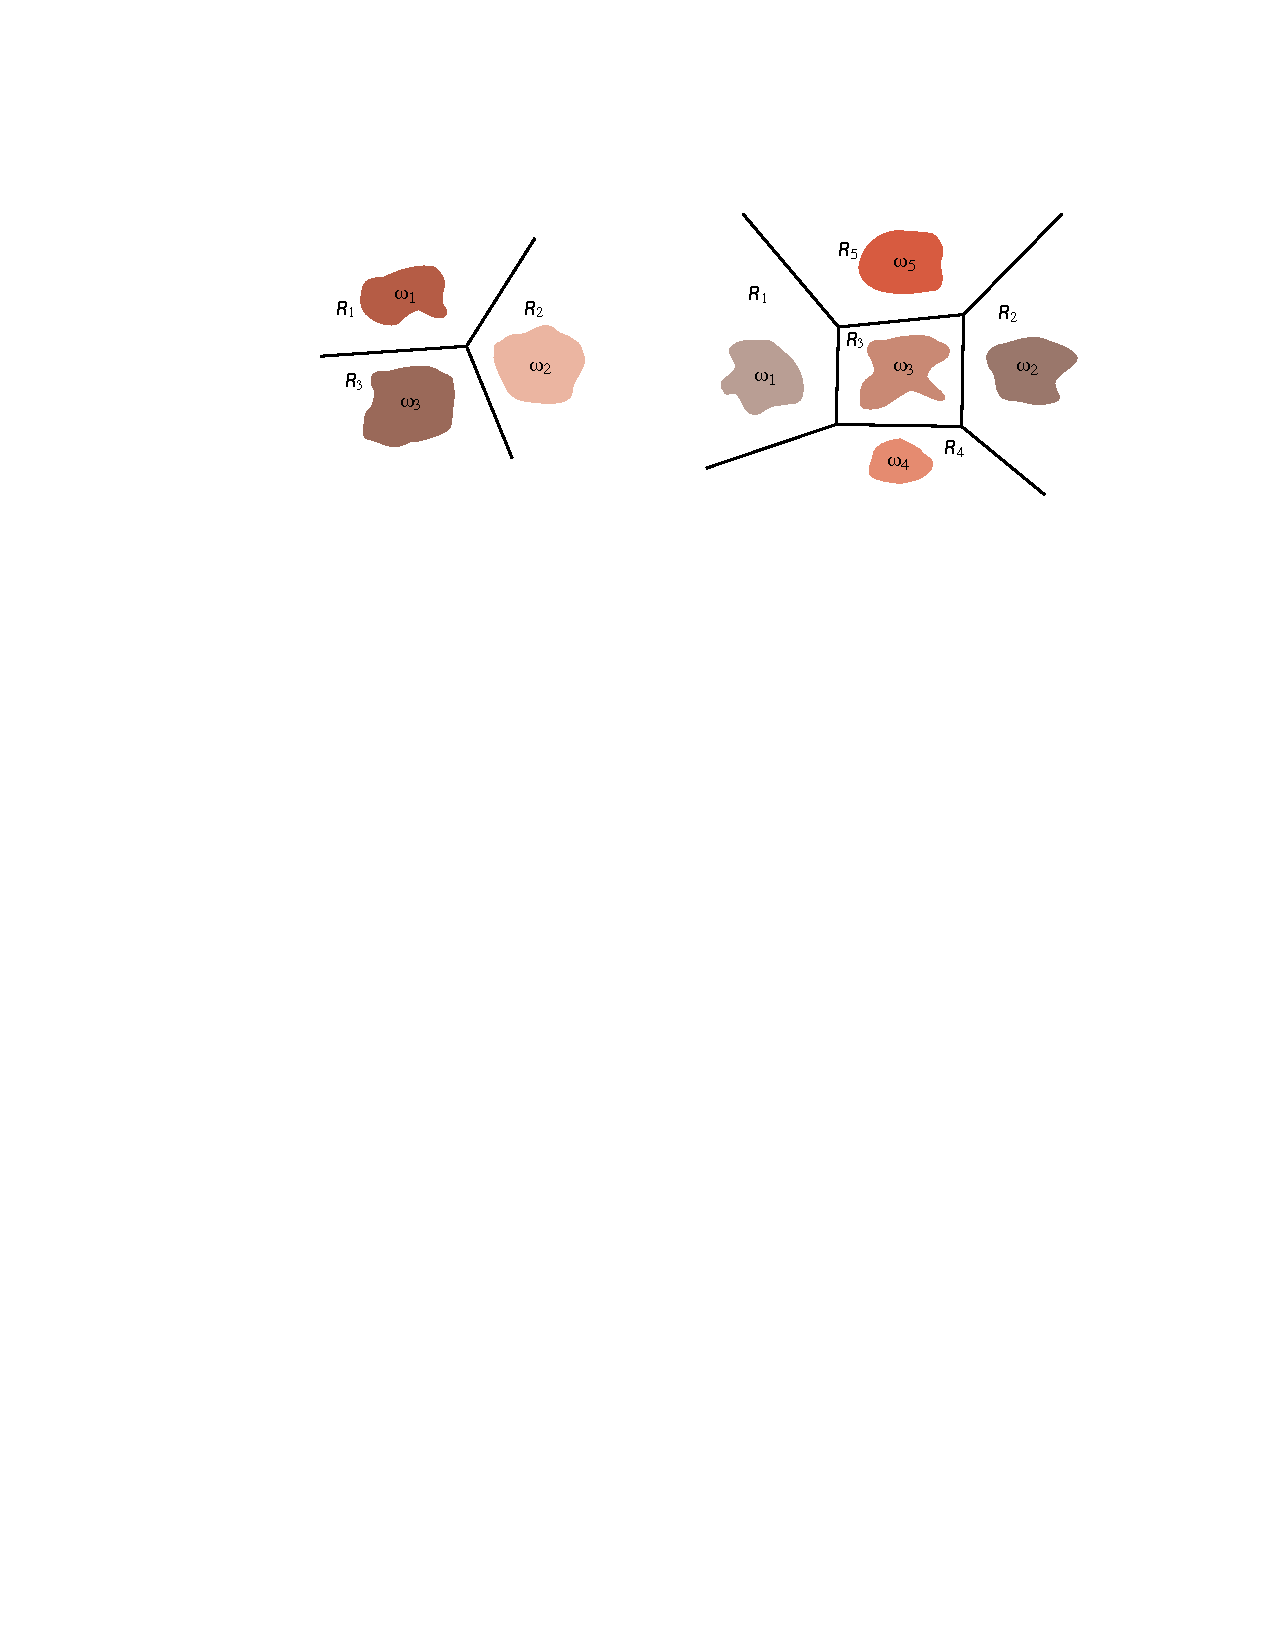
\includegraphics[width=\linewidth]{figures/ch02_linear-machine.pdf}
	\caption{Entscheidungsgrenzen erzeugt von einer \emph{linear machine} für ein Drei-Klassen- und ein Fünf-Klassen-Fall.}
	\label{fig:linear-machine}
\end{figure}

\subsubsection*{Least Squares}
\subsubsection*{Fisher's linear discriminant}
\subsubsection*{Perzeptron Algorithmus}


% -----------------------------------------------------------------------
% -----------------------------------------------------------------------
\section*{Multilayer-Perceptron (MLP)}
% -----------------------------------------------------------------------
\subsection*{Zweistufiges Perzeptron}
% Zell: Kapitel 7.4
Zweistufige binäre Perzeptrons sind mächtiger als einstufige, sie können konvexe Polygone klassifizieren. Dazu berechnen die Neuronen der ersten Ebene Hyperebenen wie im vorigen Fall auch, diese können dann aber in der zweiten Ebene durch ein Neuron, welches ein logisches AND durchführt, zum Schnitt gebracht werden, sodass sich ein konvexes Polygon ergibt.

Abbildung \ref{fig:perzeptron-zweistufig} zeigt ein Beispiel für ein zweistufiges Perzeptron und ein typisches Gebiet, dessen Punkte als Eingabe in das neuronale Netz aktzeptiert werden.

\begin{figure}[ht!] \centering 
	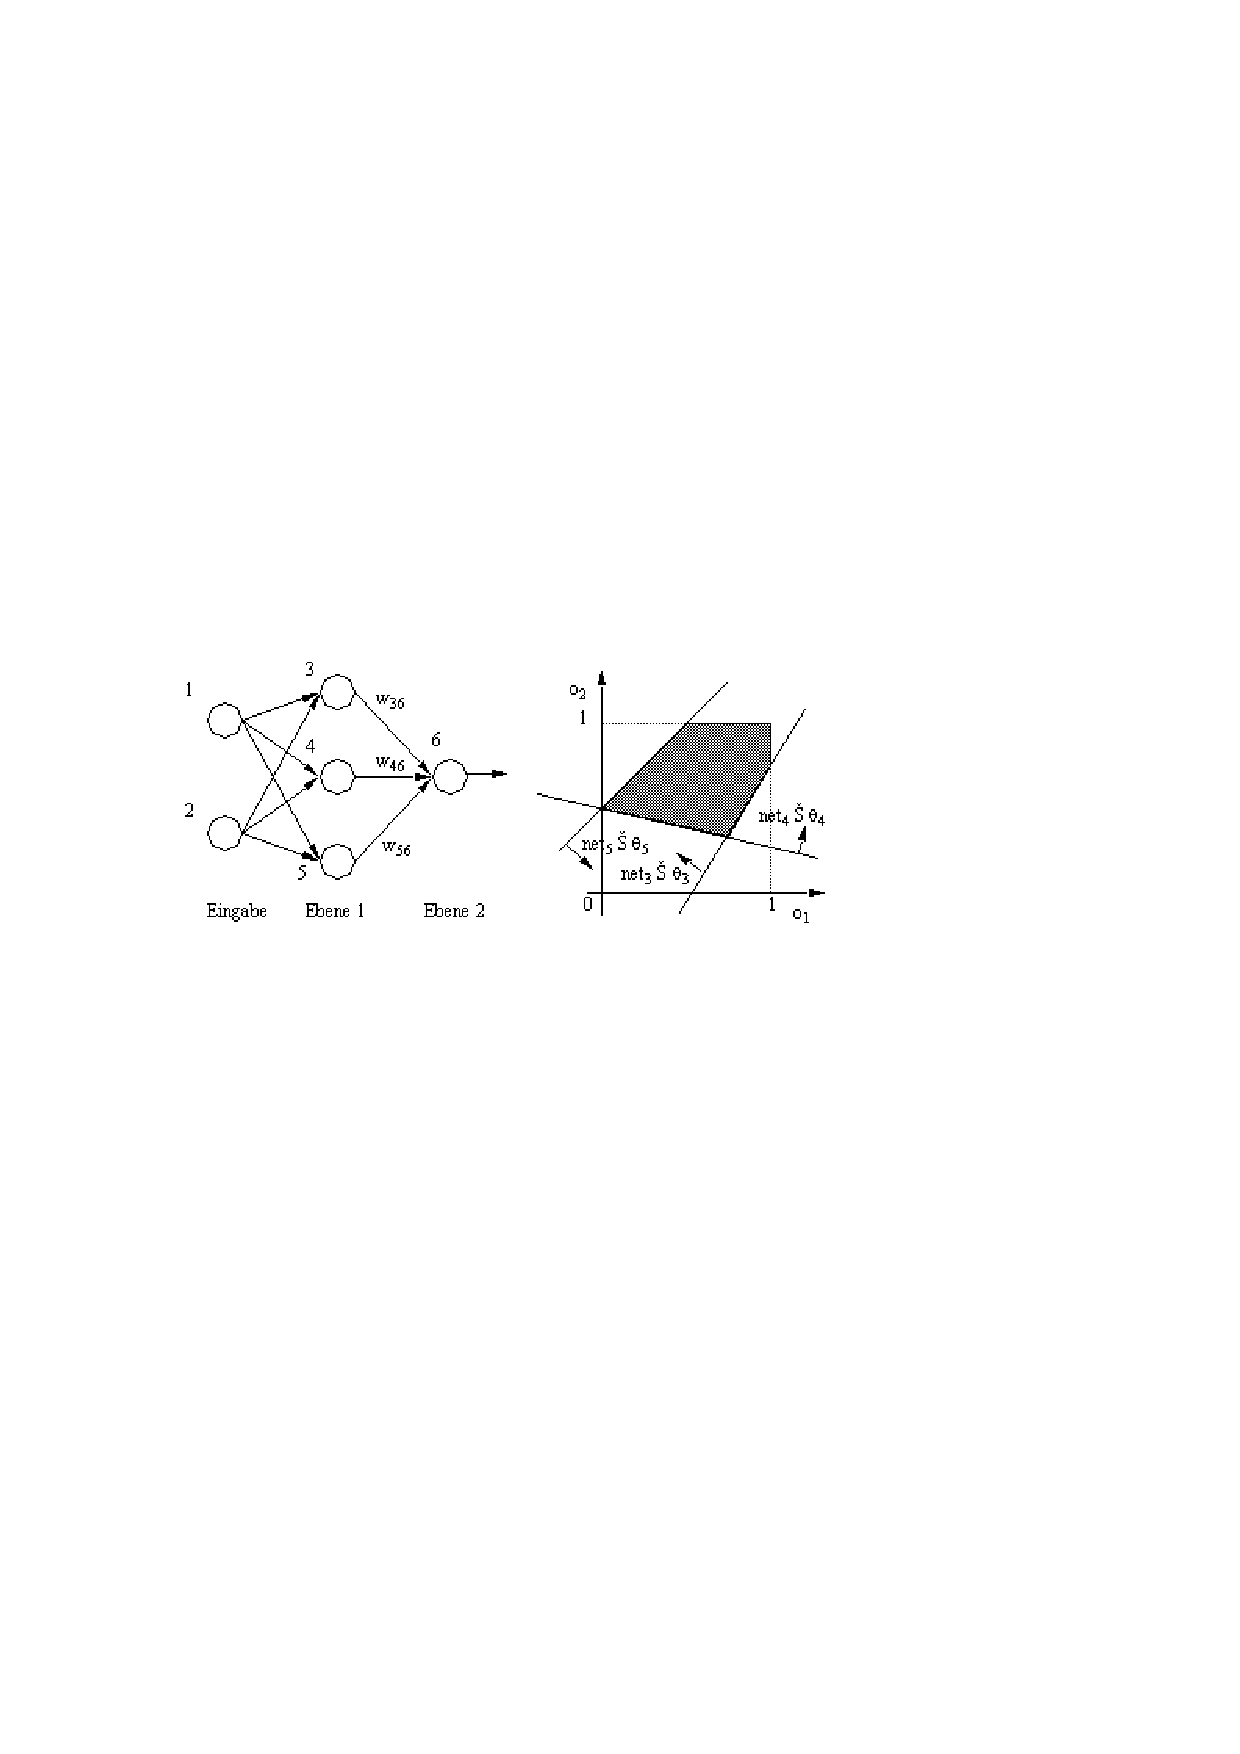
\includegraphics[width=\linewidth]{figures/ch02_perzeptron-zweistufig.pdf}
	\caption{Zweistufiges Perzeptron und ein von ihm akzeptiertes Gebiet im Merkmalsraum.}
	\label{fig:perzeptron-zweistufig}
\end{figure}

Die Funktion des logischen \emph{AND} kann dadurch erreicht werden, dass das Ausgangsneuron einen Schwellenwert besitzt, welcher der Summe der Gewichte der Verbindungen in dieses Neuron entspricht bzw. geringfügig kleiner ist:
Neuron 6 in Abbildung \ref{fig:perzeptron-zweistufig} führt durch $w_{36} = w_{46} = w_{56} = \frac{1}{3}$ und $\theta_6 = 0.9$ ein logisches AND\footnote{Die Verknüpfung der Gebiete ist nicht auf AND beschränkt. Sie könnte ebenfalls durch eine andere logische Funktion (z.B. OR, NAND, ...), welche sich mit einem einstufigen Perzeptron darstellen lässt, realisiert werden.} auf seine Eingabe durch. So wird $o_6 = 1$ genau dann, wenn $(o_1, o_2)$ im dunkel markierten konvexen Polygon liegt.

% -----------------------------------------------------------------------
\subsection*{Dreistufiges Perzeptron}
% Zell: Kapitel 7.5
Dreistufige binäre Perzeptrons können durch Überlagerung und Schnitt konvexer Polygone Mengen beliebiger Form repräsentieren. Abbildung \ref{fig:perzeptron-dreistufig} zeigt auch hierfür ein Beispiel.

\begin{figure}[ht!] \centering 
	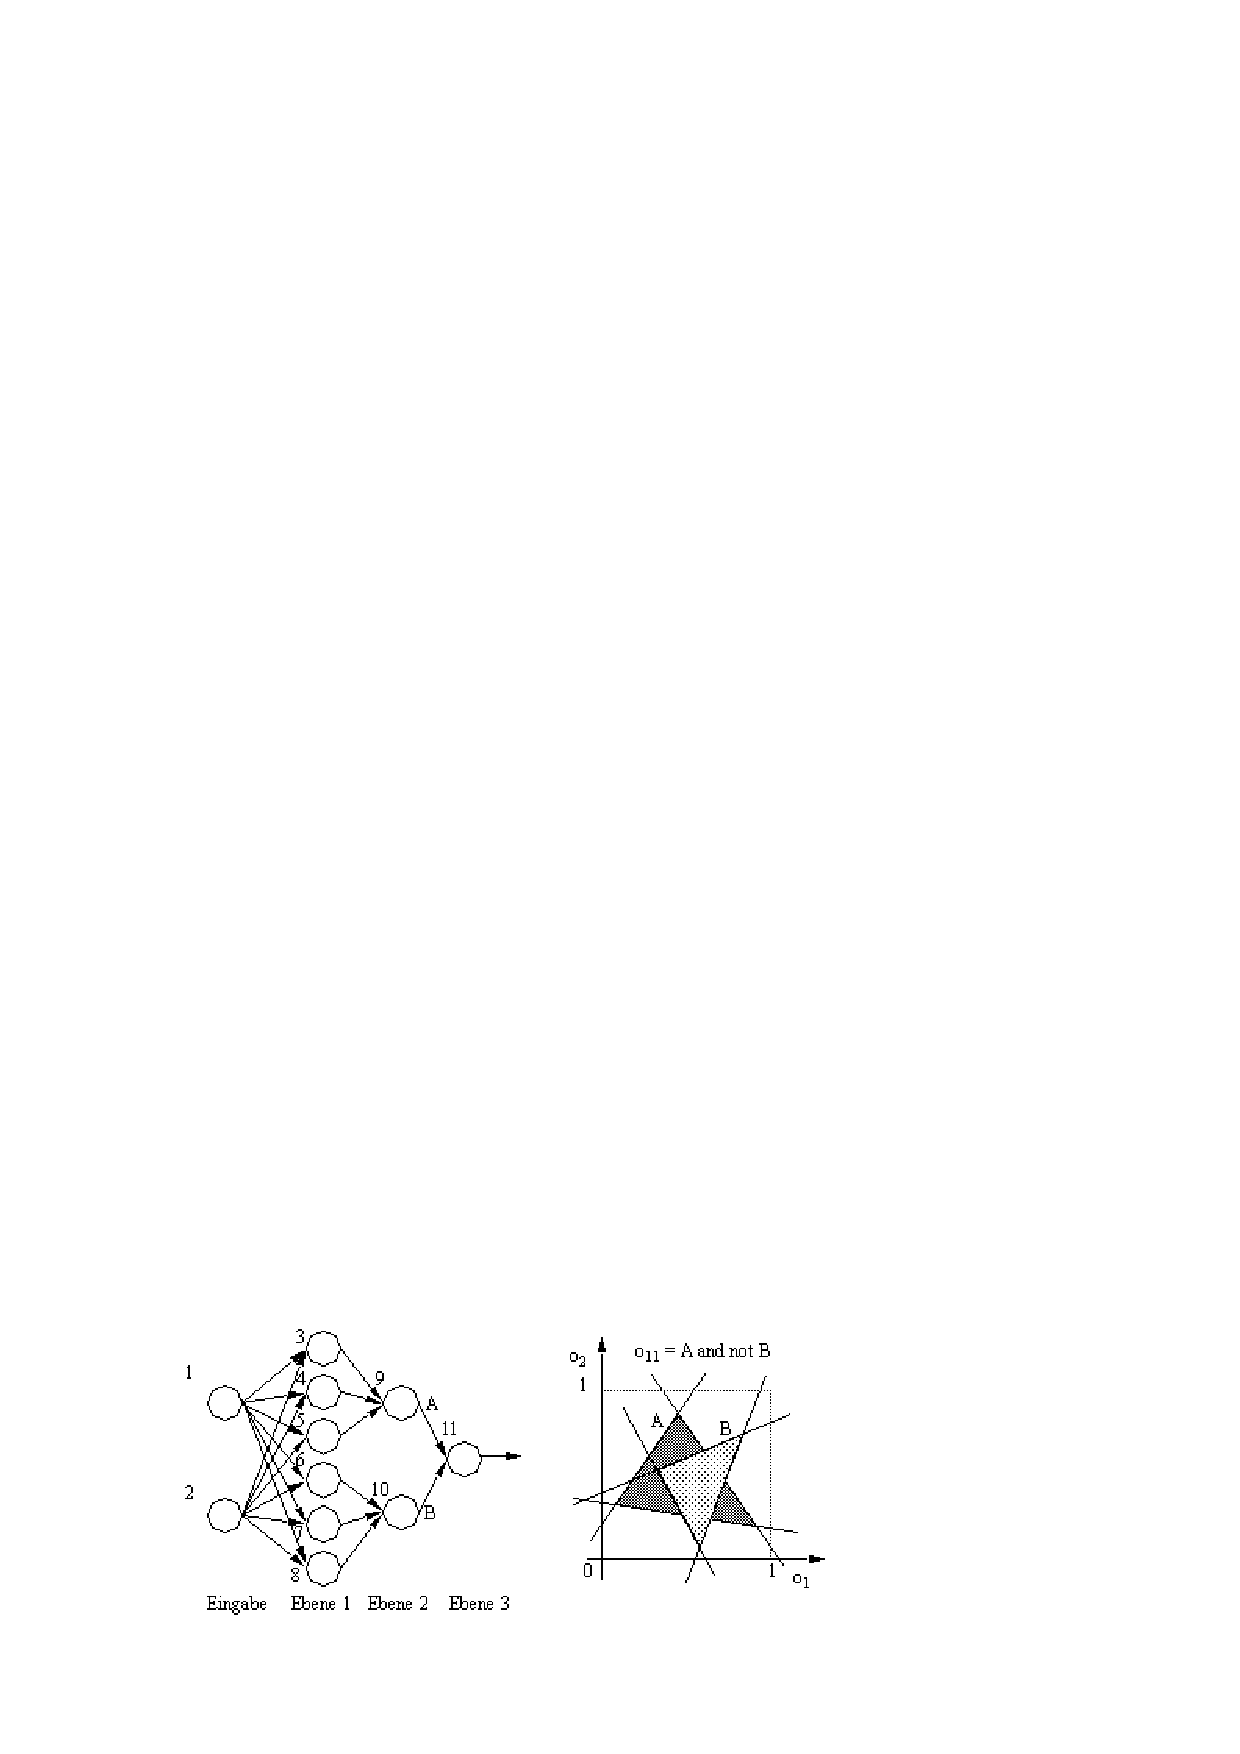
\includegraphics[width=\linewidth]{figures/ch02_perzeptron-dreistufig.pdf}
	\caption{Dreistufiges Perzeptron und ein von ihm akzeptiertes Gebiet im Merkmalsraum.}
	\label{fig:perzeptron-dreistufig}
\end{figure}

Weitere Stufen besitzen in diesem Modell keine zusätzliche Fähigkeiten mehr.


% -----------------------------------------------------------------------
% -----------------------------------------------------------------------
\section*{Perceptron Learning}
% Zell: Kapitel 7.6
\subsection*{(Rosenblatt) Perzeptron Algorithmus}
% Zell: Kapitel 7.2 (Ende)



\subsubsection*{Inverted Data Trick}

\subsubsection*{Alternative Approach}

\subsection*{Fehlerfunktionen}
\subsubsection*{Mean Squared Error (MSE)}
\subsubsection*{MSE und Sigmoid (Logistic Neuron)}

\subsection*{Softmax Group Activation Function}

\subsection*{Gradient Descent}

% ----------------------------------------------------------------------
% Themen aus Foliensatz, die in anderen Kapiteln der Zusammenfassung erläutert werden:
% ----------------------------------------------------------------------
\subsection*{McCulloch-Pitts Neuron}
% -> Wird in Kapitel 1 der Zusammenfassung erklärt.